% ==============================================================================
% Project: Topic 21 — Digital Twin-Based Early Warning System for Cold Chain
%          Disruption Detection Using Anomaly Detection
% Document: Formal Progress & Final Technical Report
% Course: Managing Corporate Entrepreneurship (B.Tech 7th Sem, 2026)
% Author: Krishna Sikheriya (Roll No: IIT2023139), B.Tech IT, IIIT Allahabad
% Supervisor: Dr. Netranand Pathak
% Target Platform: Overleaf (Compilers: pdfLaTeX / LuaLaTeX / XeLaTeX)
% ==============================================================================

\documentclass[11pt,a4paper,oneside]{article}

% ------------------------------------------------------------------------------
% 1. COLOR PALETTE
% ------------------------------------------------------------------------------
\usepackage[table,xcdraw,dvipsnames]{xcolor}
\definecolor{NavyBlue}{RGB}{14, 38, 77}       % Primary branding & section headers
\definecolor{AcademicBlue}{RGB}{2, 132, 199}   % Accent Blue & hyperlinks
\definecolor{DarkSlate}{RGB}{30, 41, 59}       % Primary body text
\definecolor{LightBlueBg}{RGB}{240, 247, 255}  % Callout box background
\definecolor{BorderGray}{RGB}{203, 213, 225}   % Table borders & dividing lines
\definecolor{HeaderGray}{RGB}{248, 250, 252}   % Table header background
\definecolor{HighlightRow}{RGB}{224, 242, 254} % Table highlight
\definecolor{EmeraldGreen}{RGB}{22, 163, 74}   % Verified / Positive metrics
\definecolor{AmberWarning}{RGB}{217, 119, 6}   % Caution / Proxy notice
\definecolor{CrimsonRed}{RGB}{220, 38, 38}     % Failure / Critical boundary
\definecolor{IceTeal}{RGB}{13, 148, 136}       % Cold-chain digital twin accent

% ------------------------------------------------------------------------------
% 2. GEOMETRY & PAGE LAYOUT
% ------------------------------------------------------------------------------
\usepackage[
    a4paper,
    top=2.4cm,
    bottom=2.4cm,
    left=2.5cm,
    right=2.5cm,
    headheight=15pt,
    headsep=0.7cm,
    footskip=1.1cm
]{geometry}

% ------------------------------------------------------------------------------
% 3. ENCODING & TYPOGRAPHY
% ------------------------------------------------------------------------------
\usepackage{iftex}
\ifpdftex
    \usepackage[T1]{fontenc}
    \usepackage[utf8]{inputenc}
    \usepackage{mathptmx}
    \usepackage[scaled=0.92]{helvet}
    \usepackage{courier}
\else
    \usepackage{fontspec}
    \setmainfont{TeX Gyre Termes}
    \setsansfont{TeX Gyre Heros}[Scale=0.94]
    \setmonofont{TeX Gyre Cursor}[Scale=0.92]
\fi

\usepackage{microtype}
\usepackage{setspace}
\setstretch{1.12}
\setlength{\parskip}{5pt plus 2pt minus 1pt}
\setlength{\parindent}{0pt}
\usepackage{enumitem}
\usepackage{etoolbox}
\usepackage{csquotes}

% ------------------------------------------------------------------------------
% 4. MATHEMATICS & UNITS
% ------------------------------------------------------------------------------
\usepackage{amsmath,mathtools}
\ifpdftex
    % mathptmx handles standard math symbols
\else
    \usepackage{amssymb}
\fi
\usepackage{siunitx}
\sisetup{group-separator={,}, group-minimum-digits=4}

% ------------------------------------------------------------------------------
% 5. GRAPHICS & CAPTIONS
% ------------------------------------------------------------------------------
\usepackage{graphicx}
\usepackage{float}
\usepackage{subcaption}
\usepackage{caption}
\captionsetup{
    font={small,rm},
    labelfont={bf,color=NavyBlue},
    labelsep=colon,
    skip=7pt,
    width=0.95\textwidth
}

% ------------------------------------------------------------------------------
% 6. TABLES
% ------------------------------------------------------------------------------
\usepackage{booktabs}
\usepackage{tabularx}
\usepackage{array}
\usepackage{makecell}
\usepackage{multirow}
\newcolumntype{L}[1]{>{\raggedright\arraybackslash}p{#1}}
\newcolumntype{C}[1]{>{\centering\arraybackslash}p{#1}}
\newcolumntype{R}[1]{>{\raggedleft\arraybackslash}p{#1}}
\newcolumntype{Y}{>{\raggedright\arraybackslash}X}
\newcolumntype{Z}{>{\centering\arraybackslash}X}

% ------------------------------------------------------------------------------
% 7. TCOLORBOX (CALLOUT CARDS)
% ------------------------------------------------------------------------------
\usepackage[most]{tcolorbox}
\tcbuselibrary{skins,breakable}

\newtcolorbox{calloutbox}[2][]{
    enhanced,
    colback=LightBlueBg,
    colframe=AcademicBlue,
    arc=3pt,
    boxrule=1.1pt,
    leftrule=4.5pt,
    fonttitle=\bfseries\color{NavyBlue}\sffamily,
    coltitle=NavyBlue,
    title={#2},
    boxsep=4pt,
    left=8pt,
    right=8pt,
    top=6pt,
    bottom=6pt,
    breakable,
    #1
}

\newtcolorbox{cautionbox}[2][]{
    enhanced,
    colback=AmberWarning!6!white,
    colframe=AmberWarning!90!black,
    arc=3pt,
    boxrule=1.1pt,
    leftrule=4.5pt,
    fonttitle=\bfseries\color{white}\sffamily,
    colbacktitle=AmberWarning!90!black,
    coltitle=white,
    title={#2},
    boxsep=4pt,
    left=8pt,
    right=8pt,
    top=6pt,
    bottom=6pt,
    breakable,
    #1
}

% ------------------------------------------------------------------------------
% 8. TIKZ DIAGRAMS & FLOWCHARTS
% ------------------------------------------------------------------------------
\usepackage{tikz}
\usetikzlibrary{shapes.geometric, arrows.meta, positioning, calc, fit, backgrounds, shadows, decorations.pathreplacing}

\tikzset{
    flowblock/.style={
        rectangle,
        draw=NavyBlue,
        fill=white,
        thick,
        rounded corners=2pt,
        text centered,
        font=\small\sffamily,
        minimum height=0.9cm,
        minimum width=2.4cm,
        drop shadow={opacity=0.15, shadow xshift=1pt, shadow yshift=-1pt}
    },
    accentblock/.style={
        rectangle,
        draw=AcademicBlue,
        fill=LightBlueBg,
        thick,
        rounded corners=2pt,
        text centered,
        font=\small\sffamily\bfseries,
        minimum height=0.9cm,
        minimum width=2.5cm,
        drop shadow={opacity=0.15, shadow xshift=1pt, shadow yshift=-1pt}
    },
    twinblock/.style={
        rectangle,
        draw=IceTeal!90!black,
        fill=IceTeal!8!white,
        thick,
        rounded corners=3pt,
        text centered,
        font=\small\sffamily\bfseries,
        minimum height=1.0cm,
        minimum width=2.6cm,
        drop shadow={opacity=0.18, shadow xshift=1pt, shadow yshift=-1pt}
    },
    monitorblock/.style={
        rectangle,
        draw=NavyBlue!90,
        fill=HeaderGray,
        thick,
        rounded corners=2pt,
        text centered,
        font=\footnotesize\sffamily,
        minimum height=0.8cm,
        minimum width=2.2cm
    },
    flowarrow/.style={
        -{Stealth[scale=1.1]},
        thick,
        draw=NavyBlue!80
    },
    dashedarrow/.style={
        -{Stealth[scale=1.0]},
        thick,
        dashed,
        draw=AcademicBlue
    }
}

% ------------------------------------------------------------------------------
% 9. HEADERS & FOOTERS (FANCYHDR)
% ------------------------------------------------------------------------------
\usepackage{fancyhdr}
\pagestyle{fancy}
\fancyhf{}
\renewcommand{\headrulewidth}{0.5pt}
\renewcommand{\headrule}{\hbox to\headwidth{\color{BorderGray}\leaders\hrule height \headrulewidth\hfill}}
\fancyhead[L]{\small\sffamily\color{DarkSlate}Topic 21 — Digital Twin Cold Chain Early Warning System}
\fancyhead[R]{\small\sffamily\color{AcademicBlue}\textbf{Progress Report}}
\fancyfoot[C]{\small\sffamily\color{DarkSlate}\thepage}
\fancyfoot[R]{\scriptsize\sffamily\color{BorderGray!80!black}IIIT Allahabad}

% ------------------------------------------------------------------------------
% 10. SECTION FORMATTING (TITLESEC)
% ------------------------------------------------------------------------------
\usepackage{titlesec}
\titleformat{\section}
    {\normalfont\sffamily\Large\bfseries\color{NavyBlue}}
    {\thesection}{0.8em}{}
    [\vspace{-2pt}\color{AcademicBlue}\hrule height 0.8pt]

\titleformat{\subsection}
    {\normalfont\sffamily\large\bfseries\color{NavyBlue!90!black}}
    {\thesubsection}{0.6em}{}

\titleformat{\subsubsection}
    {\normalfont\sffamily\normalsize\bfseries\color{DarkSlate}}
    {\thesubsubsection}{0.5em}{}

\titlespacing*{\section}{0pt}{14pt}{8pt}
\titlespacing*{\subsection}{0pt}{10pt}{5pt}
\titlespacing*{\subsubsection}{0pt}{7pt}{3pt}

% ------------------------------------------------------------------------------
% 11. HYPERLINKS & BIBLIOGRAPHY
% ------------------------------------------------------------------------------
\usepackage{hyperref}
\hypersetup{
    colorlinks=true,
    linkcolor=NavyBlue,
    citecolor=AcademicBlue,
    filecolor=NavyBlue,
    urlcolor=AcademicBlue,
    pdfauthor={Krishna Sikheriya (IIT2023139)},
    pdftitle={Topic 21: Digital Twin-Based Early Warning System for Cold Chain Disruption Detection},
    pdfsubject={Progress Report — Managing Corporate Entrepreneurship, IIIT Allahabad}
}
\usepackage[nameinlink,capitalize,noabbrev]{cleveref}

\usepackage[
    backend=biber,
    style=authoryear,
    sorting=nyt,
    maxcitenames=2,
    mincitenames=1,
    maxbibnames=6,
    doi=true,
    url=false
]{biblatex}
\addbibresource{references.bib}

% ==============================================================================
% DOCUMENT BODY
% ==============================================================================
\begin{document}

% ------------------------------------------------------------------------------
% TITLE BLOCK & INSTITUTIONAL HEADER
% ------------------------------------------------------------------------------
\begin{center}
    \begin{minipage}{0.18\textwidth}
        \centering
        
\includegraphics[height=2.2cm]{figures/iiit_allahabad_logo.png}
    \end{minipage}
    \hfill
    \begin{minipage}{0.80\textwidth}
        \raggedright
        {\LARGE\bfseries\color{NavyBlue}\sffamily Indian Institute of Information Technology, Allahabad}\\[3pt]
        {\large\bfseries\color{AcademicBlue}\sffamily Department of Information Technology}\\[2pt]
        {\small\color{DarkSlate}\textbf{Course:} Managing Corporate Entrepreneurship (B.Tech 7th Semester, 2026)}\\[2pt]
        {\small\color{DarkSlate}\textbf{Supervisor / Instructor:} Dr. Netranand Pathak}
    \end{minipage}
\end{center}

\vspace{-4pt}
\textcolor{AcademicBlue}{\hrule height 1.5pt}
\vspace{6pt}

\begin{center}
    {\Large\bfseries\color{NavyBlue}\sffamily Topic 21: Digital Twin-Based Early Warning System for Cold Chain Disruption Detection Using Anomaly Detection}\\[4pt]
    {\large\sffamily Comprehensive Progress \& Final Technical Milestone Report}\\[6pt]
    \textbf{Student Author:} Krishna Sikheriya \quad $\vert$ \quad \textbf{Roll Number:} IIT2023139\\[2pt]
    \textbf{Repository:} \href{https://github.com/Krishna200608/coldchain-ews-twin}{\texttt{github.com/Krishna200608/coldchain-ews-twin}} \quad $\vert$ \quad
    \textbf{Live Web App:} \href{https://coldchain-ews-twin.streamlit.app/}{\texttt{coldchain-ews-twin.streamlit.app}}
\end{center}

\vspace{4pt}

% ------------------------------------------------------------------------------
% SECTION 1: EXECUTIVE SUMMARY
% ------------------------------------------------------------------------------
\section{Executive Summary \& Project Status}

Cold-chain logistics for pharmaceuticals, biologics, and premium perishable food commodities demand unbroken thermal control across multi-echelon transit. Existing commercial logistics platforms depend heavily on \textbf{static threshold alarms} (e.g., triggering only after ambient temperature breaches $+8^\circ\text{C}$ continuously for 10--15 minutes). Under real operating conditions, cumulative thermal exposure degrades sensitive active ingredients long before static tripwires trigger, rendering conventional alarms fundamentally reactive.

This project designs, validates, and deploys a complete \textbf{Digital Twin-Integrated Early Warning System (EWS)}. By embedding unsupervised and deep sequential anomaly detectors directly inside an event-driven discrete-event digital twin (SimPy), the system identifies subtle precursor degradation patterns—such as mechanical compressor refrigeration drift and sensor variance collapses—prior to irreversible thermal damage.

\begin{calloutbox}{Project Status: 100\% Complete and Fully Verified}
The project has fulfilled 100\% of the technical and empirical specifications established by the supervisor. Every pipeline component—from causal feature preprocessing, controlled anomaly injection, and model inference, to the 3-stage SimPy digital twin simulation loop, automated cross-check suites, and public interactive web dashboard—is implemented, verified with zero mismatches, and tracked in open-source version control.
\end{calloutbox}

% ------------------------------------------------------------------------------
% SECTION 2: RESEARCH GAP, OBJECTIVES & FORMAL RESEARCH QUESTIONS
% ------------------------------------------------------------------------------
\section{Research Gap, Core Objectives \& Research Questions}

\subsection{The Academic Literature Gap}
Traditional cold-chain monitoring research focuses on post-hoc spoilage and shelf-life modeling (e.g., calculating Arrhenius kinetic degradation after excursions have already concluded). Meanwhile, industrial digital twins focus primarily on predictive maintenance of stationary machinery. Embedding machine-learning anomaly detection into an event-driven cold-chain digital twin to deliver quantifiable, pre-failure early warning runway ($\Delta t_{\text{lead}}$) remains markedly underexplored in peer-reviewed literature.

\subsection{Core Objectives}
\begin{enumerate}[leftmargin=1.8em, itemsep=2pt, topsep=2pt]
    \item \textbf{Causal Digital Twin Architecture:} Develop a three-stage discrete-event simulation (\texttt{Source} $\rightarrow$ \texttt{Transit} $\rightarrow$ \texttt{Destination}) in SimPy modeling physical transit and realistic irregular sensor arrival dynamics.
    \item \textbf{Embedded Model Comparison:} Embed both a classical tree partition ensemble (\textbf{Isolation Forest}) and a deep temporal reconstruction network (\textbf{LSTM-Autoencoder}) into the streaming twin sink.
    \item \textbf{Empirical Lead-Time Quantification:} Quantify the exact early warning runway ($\Delta t_{\text{lead}} = t_{\text{irr}} - t_{\text{alarm}}$) achieved across diverse disruption categories relative to static threshold alarms.
    \item \textbf{Simulation Parity Verification:} Prove that live discrete-event evaluation matches offline batch evaluation bit-for-bit without cold-start divergence or look-ahead leakage.
\end{enumerate}

\subsection{Resolution of Research Questions}
\begin{table}[H]
\centering
\small
\renewcommand{\arraystretch}{1.25}
\begin{tabularx}{\textwidth}{L{3.2cm} Y C{2.2cm}}
\toprule
\rowcolor{HeaderGray}
\textbf{Research Question} & \textbf{Empirical Resolution \& Findings} & \textbf{Status} \\
\midrule
\textbf{RQ1: Early-Warning Lead Time}\newline\textit{Can models flag disruptions before irreversibility, and how early?} &
Isolation Forest provides substantial, actionable lead time on gradual drift disruptions: \textbf{+64.0 minutes} on ambient (\texttt{Out}) and \textbf{+11.0 minutes} on enclosure (\texttt{In}). For sudden step jumps, all detectors trigger concurrently ($0.0$ min runway). For sensor flatlines, threshold alarms fail completely, while Isolation Forest successfully triggers. &
\textbf{\textcolor{EmeraldGreen}{Resolved}} (Table~\ref{tab:lead_times}) \\
\addlinespace
\textbf{RQ2: Classical vs.\ Deep Learning}\newline\textit{How do tree ensembles compare against sequential autoencoders?} &
\textbf{Isolation Forest} acts as an aggressive, high-recall tripwire ($80.0\%$ \texttt{Out}, $91.3\%$ \texttt{In}), accepting elevated false-positive rates ($45.6\%$). \textbf{LSTM-Autoencoder} is highly conservative on \texttt{In} ($2.85\%$ FPR, $13.1\%$ precision), but experiences temporal adaptation lag on \texttt{Out} drift (late by $14.0$ min). &
\textbf{\textcolor{EmeraldGreen}{Resolved}} (Table~\ref{tab:pointwise_metrics}) \\
\addlinespace
\textbf{RQ3: Digital Twin Simulation Fidelity}\newline\textit{Does embedding in an event loop cause silent divergence?} &
\textbf{100\% Bit-for-Bit Parity:} SimPy replayed \num{97603} telemetry events in \SI{6.03}{\second} ($>1.9\times 10^6$ speedup) with \textbf{\SI{0.00}{\second}} timing discrepancy. Across 30 injections $\times$ 3 monitors, all 42 applicable test evaluations matched batch evaluations identically (0 mismatches), guaranteed via buffer pre-warming. &
\textbf{\textcolor{EmeraldGreen}{Resolved}} (\texttt{twin\_crosscheck}) \\
\bottomrule
\end{tabularx}
\caption{Summary of Core Research Questions and Empirical Findings.}
\label{tab:rq_summary}
\end{table}

% ------------------------------------------------------------------------------
% SECTION 3: RELEVANT LITERATURE REVIEW
% ------------------------------------------------------------------------------
\section{Relevant Literature Review \& Benchmark Foundations}

Our study is situated within the contemporary literature on industrial digital twins, IoT telemetry streaming, and machine-learning anomaly detection for supply chains (2023--2026):

\begin{table}[H]
\centering
\small
\renewcommand{\arraystretch}{1.2}
\begin{tabularx}{\textwidth}{L{3.0cm} L{3.5cm} Y Y}
\toprule
\rowcolor{HeaderGray}
\textbf{Study} & \textbf{Publication Venue} & \textbf{Core Contribution} & \textbf{Direct Relevance to Our Project} \\
\midrule
\textbf{\citet{vuksic2026early}} & \textit{Applied Sciences} (MDPI) & Hybrid physics-based digital twin + autoencoder for reefer maritime containers. & Reports median early warning lead time of \textbf{\~{}68 minutes}, directly corroborating our \textbf{64.0-minute} drift lead time. \\
\addlinespace
\textbf{\citet{xie2025anomaly}} & \textit{PLOS ONE} & Improved Isolation Forest (subsampling + feature cross-grouping) for cold-chain fleet streams. & Primary tree-ensemble benchmark for cold-chain streaming; contextualizes point-wise F1 metrics under extreme anomaly rarity. \\
\addlinespace
\textbf{\citet{meng2024costeffective}} & \textit{Journal of Food Engineering} (Elsevier) & Box-level digital twin temperature modeling + static over-temperature alarms. & Exemplifies the static threshold-alarm paradigm our proactive anomaly-detection system benchmarks against. \\
\addlinespace
\textbf{\citet{wu2023internet}} & \textit{J.\ Industrial Information Integration} & Internet-of-Everything and Digital-Twin platform for cold-chain visibility. & Establishes architectural precedent for embedding AI inference into operational digital-twin pipelines. \\
\addlinespace
\textbf{\citet{defraeye2023digital}} & \textit{Comput.\ Electron.\ Agric.} / \textit{J.\ Food Eng.} & State-of-the-art review of food cold-chain digital twins. & Formulates the primary research gap: transitioning from post-hoc quality loss to live event-driven anomaly early warning. \\
\addlinespace
\textbf{\citet{liu2008isolation}} & \textit{IEEE ICDM} & Foundational tree-partition anomaly isolation algorithm. & Theoretical basis for our embedded \texttt{IFMonitor}. \\
\addlinespace
\textbf{\citet{malhotra2016lstm}} & \textit{ICML Workshop} & Sequential encoder-decoder LSTM reconstruction architecture. & Foundation for our bivariate sequential \texttt{LSTMMonitor}. \\
\bottomrule
\end{tabularx}
\caption{Recent Literature Review and Theoretical Benchmark Foundations.}
\label{tab:literature_review}
\end{table}

% ------------------------------------------------------------------------------
% SECTION 4: DATA STRATEGY & STRUCTURAL PROXY NOTICE
% ------------------------------------------------------------------------------
\section{Data Strategy, Irregular Telemetry \& Structural-Proxy Notice}

\subsection{Dataset Ingestion and Sampling Dynamics}
The empirical pipeline processes the Kaggle IoT temperature dataset (\texttt{IOT-temp.csv}, \SI{6.63}{\mega\byte}, \num{97606} raw readings) spanning July 28, 2018 to December 8, 2018 (133 continuous days, \num{27920} unique minute timestamps). As shown in \cref{fig:temp_and_sampling}, the data exhibits severe telemetry irregularities:
\begin{itemize}[leftmargin=1.5em, itemsep=2pt, topsep=1pt]
    \item \textbf{High Burstiness \& Irregular Arrival:} Mean inter-arrival gap $\Delta t = \SI{117.82}{\second}$, median $\Delta t = \SI{0.0}{\second}$, standard deviation $\sigma_{\Delta t} = \SI{5446.3}{\second}$, yielding an extreme Coefficient of Variation $\text{CoV} = 46.23$. Network dropouts create outages of up to 11.57 days.
    \item \textbf{Dual Telemetry Streams:} Data is split by physical enclosure tag: ambient (\texttt{Out}, \num{77260} rows) and refrigerated container proxy (\texttt{In}, \num{20345} rows).
\end{itemize}

\begin{figure}[H]
    \centering
    \begin{subfigure}[b]{0.48\textwidth}
        \centering
        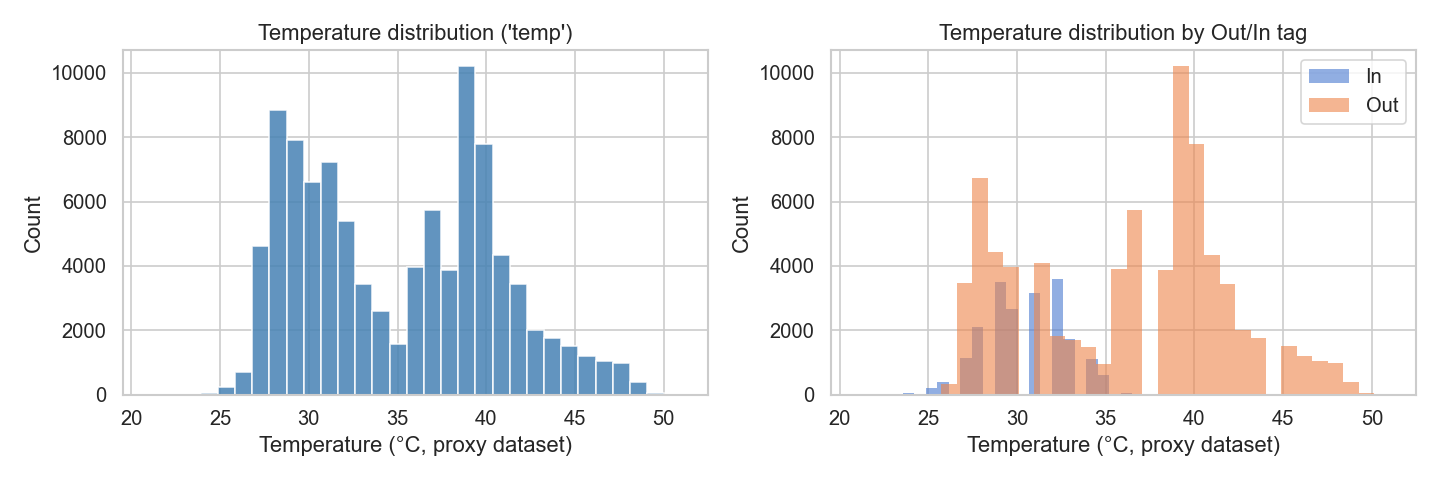
\includegraphics[width=\textwidth]{figures/fig_temperature_distribution.png}
        \caption{Temperature Distribution (\texttt{In} vs.\ \texttt{Out}).}
        \label{fig:temp_dist}
    \end{subfigure}
    \hfill
    \begin{subfigure}[b]{0.48\textwidth}
        \centering
        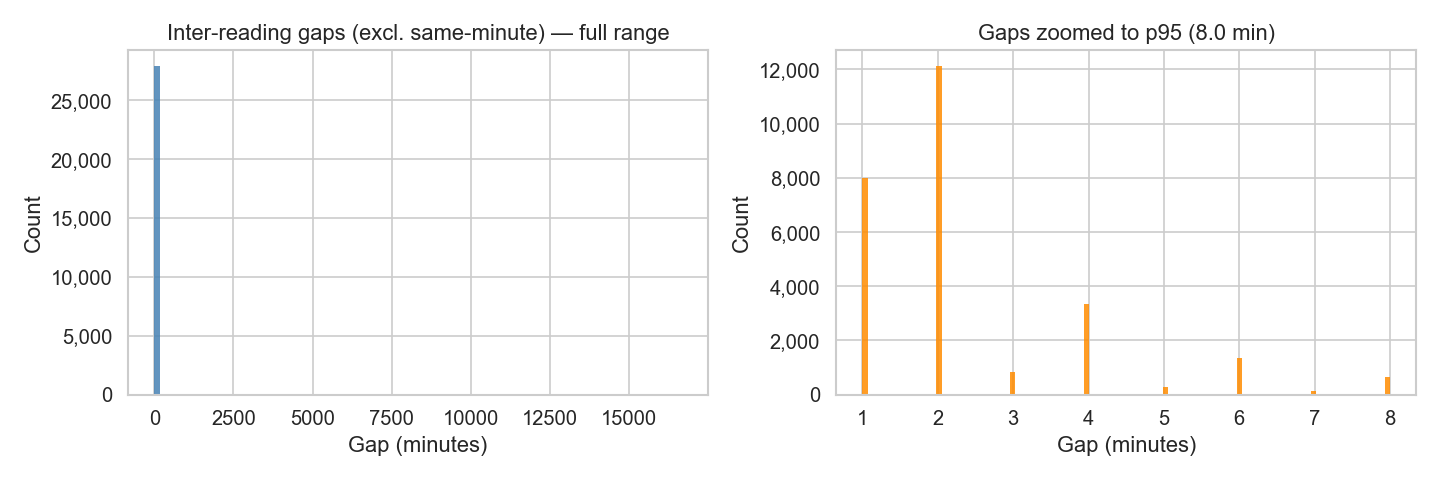
\includegraphics[width=\textwidth]{figures/fig_sampling_intervals_corrected.png}
        \caption{Log-Scale Inter-Arrival Time Gaps ($\Delta t_k$).}
        \label{fig:sampling_dist}
    \end{subfigure}
    \caption{Empirical Telemetry Properties of the Kaggle IoT Temperature Dataset.}
    \label{fig:temp_and_sampling}
\end{figure}

\begin{cautionbox}{Academic Integrity: Structural-Proxy Framing Notice}
In accordance with strict scientific integrity, this dataset originates from a building administration installation (\texttt{room\_id/id = "Room Admin"}), not active pharmaceutical reefer vehicles. In this project, it is framed strictly as an experimental \textbf{structural proxy} to evaluate irregular streaming pipelines, buffer synchronization, and embedded inference architectures without fabricating claims of clinical field trials.
\end{cautionbox}

% ------------------------------------------------------------------------------
% SECTION 5: METHODOLOGY & DIGITAL TWIN SYSTEM ARCHITECTURE
% ------------------------------------------------------------------------------
\section{Methodology and System Architecture}

\subsection{End-to-End System Flowchart (TikZ)}
The system architecture integrates physical data ingestion, causal stream preprocessing, controlled perturbation injection, discrete-event simulation, and real-time early warning monitors (\cref{fig:tikz_pipeline}).

\begin{figure}[H]
\centering
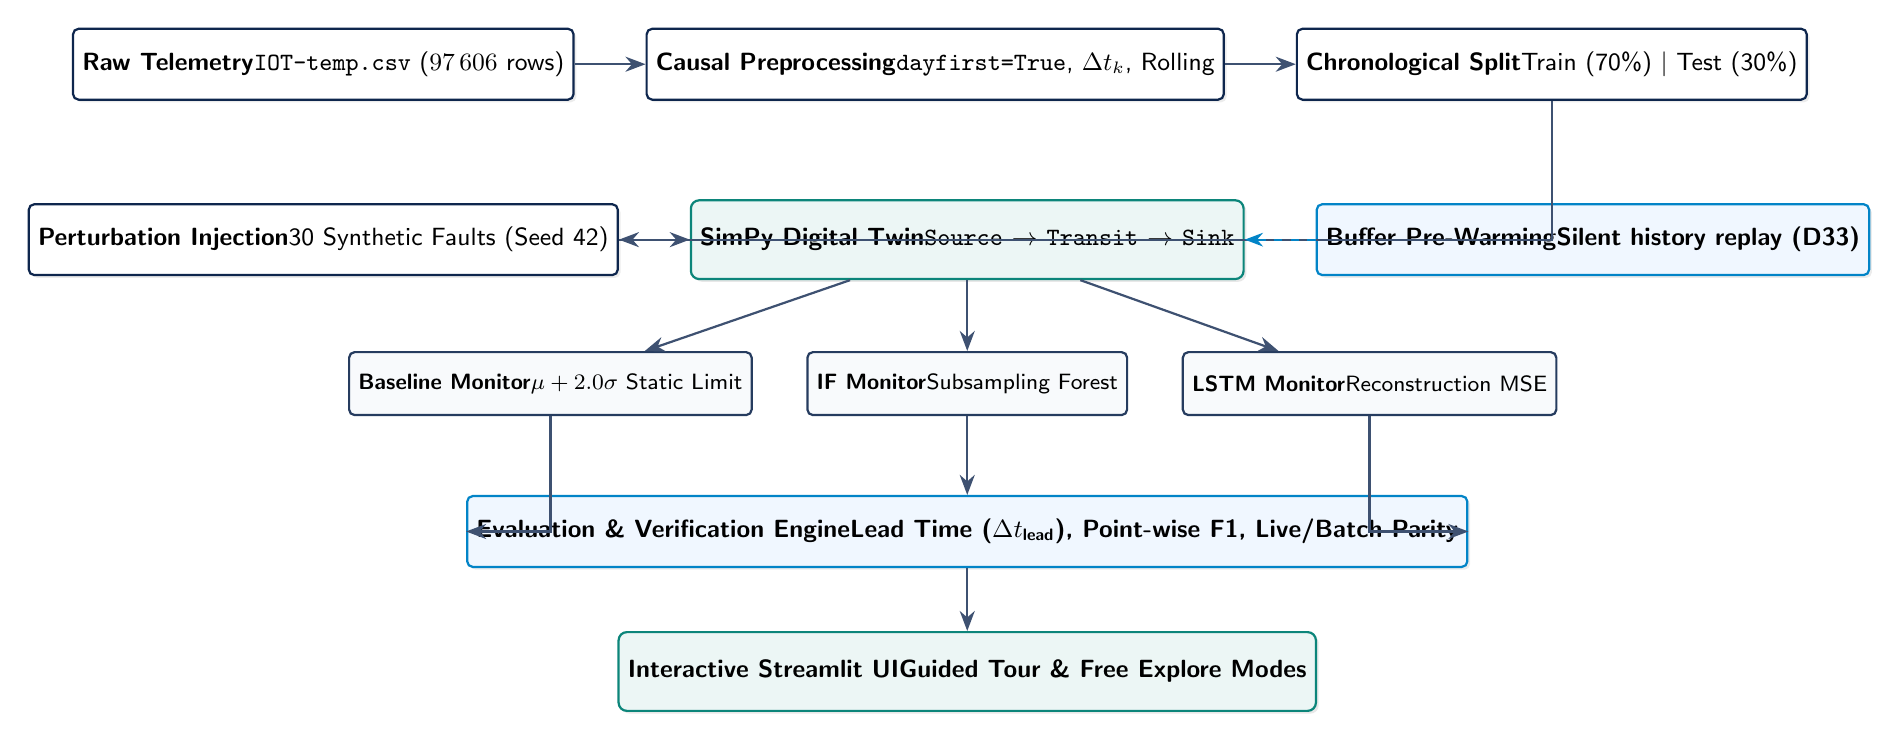
\begin{tikzpicture}[node distance=1.3cm and 0.9cm]

    % Row 1: Physical Data & Preprocessing
    \node (raw) [flowblock] {\textbf{Raw Telemetry}\\ \texttt{IOT-temp.csv} (\num{97606} rows)};
    \node (prep) [flowblock, right=of raw] {\textbf{Causal Preprocessing}\\ \texttt{dayfirst=True}, $\Delta t_k$, Rolling};
    \node (split) [flowblock, right=of prep] {\textbf{Chronological Split}\\ Train (70\%) $\vert$ Test (30\%)};

    % Row 2: Perturbation Protocol & SimPy Digital Twin
    \node (inject) [flowblock, below=of raw] {\textbf{Perturbation Injection}\\ 30 Synthetic Faults (Seed 42)};
    \node (simpy) [twinblock, right=of inject, minimum width=3.0cm] {\textbf{SimPy Digital Twin}\\ \texttt{Source} $\rightarrow$ \texttt{Transit} $\rightarrow$ \texttt{Sink}};
    \node (prewarm) [accentblock, right=of simpy] {\textbf{Buffer Pre-Warming}\\ Silent history replay (D33)};

    % Row 3: Embedded Streaming Monitors
    \node (mon_base) [monitorblock, below left=0.9cm and -0.8cm of simpy] {\textbf{Baseline Monitor}\\ $\mu + 2.0\sigma$ Static Limit};
    \node (mon_if) [monitorblock, below=0.9cm of simpy] {\textbf{IF Monitor}\\ Subsampling Forest};
    \node (mon_lstm) [monitorblock, below right=0.9cm and -0.8cm of simpy] {\textbf{LSTM Monitor}\\ Reconstruction MSE};

    % Row 4: Outputs
    \node (eval) [accentblock, below=1.0cm of mon_if, minimum width=4.5cm] {\textbf{Evaluation \& Verification Engine}\\ Lead Time ($\Delta t_{\text{lead}}$), Point-wise F1, Live/Batch Parity};
    \node (dash) [twinblock, below=0.8cm of eval, minimum width=4.5cm] {\textbf{Interactive Streamlit UI}\\ Guided Tour \& Free Explore Modes};

    % Arrows
    \draw [flowarrow] (raw) -- (prep);
    \draw [flowarrow] (prep) -- (split);
    \draw [flowarrow] (split) |- (inject);
    \draw [flowarrow] (inject) -- (simpy);
    \draw [dashedarrow] (prewarm) -- (simpy);
    
    \draw [flowarrow] (simpy) -- (mon_base);
    \draw [flowarrow] (simpy) -- (mon_if);
    \draw [flowarrow] (simpy) -- (mon_lstm);

    \draw [flowarrow] (mon_base) |- (eval);
    \draw [flowarrow] (mon_if) -- (eval);
    \draw [flowarrow] (mon_lstm) |- (eval);

    \draw [flowarrow] (eval) -- (dash);

\end{tikzpicture}
\caption{TikZ Flowchart: End-to-End Digital Twin Early Warning Architecture.}
\label{fig:tikz_pipeline}
\end{figure}

\subsection{Controlled Synthetic Anomaly Protocol}
To benchmark detectors under controlled ground truth, 30 synthetic perturbations were seeded across the timeline (\texttt{RANDOM\_SEED = 42}) across three canonical failure modes:
\begin{enumerate}[leftmargin=1.5em, itemsep=1pt, topsep=1pt]
    \item \textbf{Step Disruptions (10):} Instantaneous temperature jump ($+5^\circ\text{C}$ to $+15^\circ\text{C}$), modeling container doors left open or acute refrigeration power loss.
    \item \textbf{Linear Drift Disruptions (10):} Slow ramp-up ($+0.05^\circ\text{C}$ to $+0.25^\circ\text{C}$ per minute), modeling progressive coolant leaks or mechanical compressor wear.
    \item \textbf{Sensor Flatline Disruptions (10):} Zero variance persistence, modeling frozen analog-to-digital converter sensors or telemetry stiction.
\end{enumerate}

\begin{figure}[H]
    \centering
    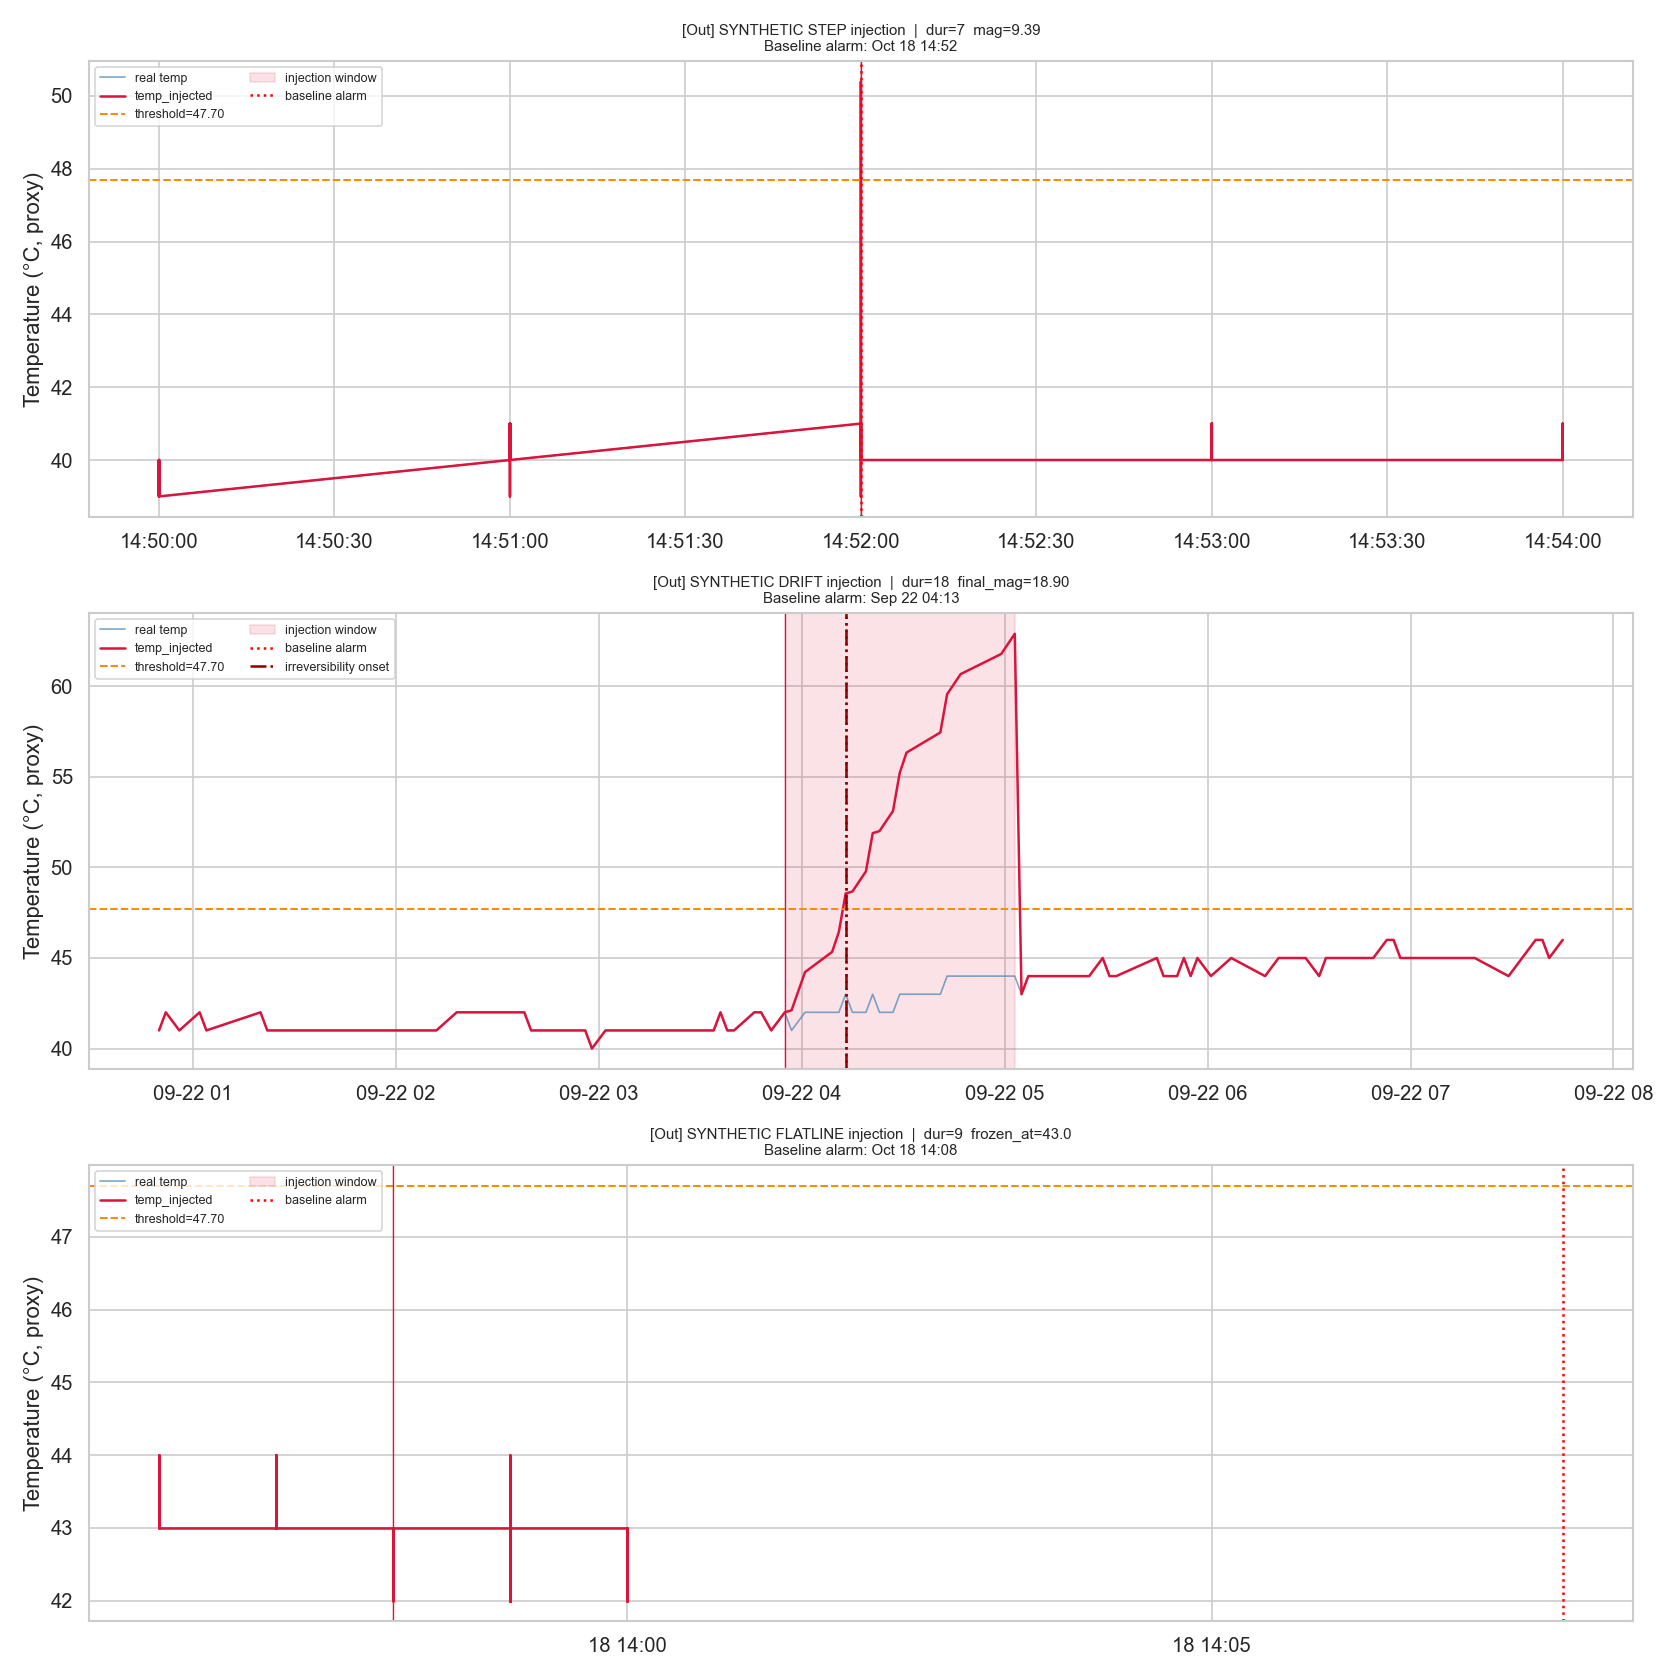
\includegraphics[width=0.92\textwidth]{figures/fig_injection_examples.png}
    \caption{Controlled Synthetic Perturbation Profiles: Step Spikes, Linear Drifts, and Sensor Flatlines.}
    \label{fig:injection_examples}
\end{figure}

\subsection{Embedded Anomaly Detection Models}
\begin{itemize}[leftmargin=1.5em, itemsep=3pt, topsep=2pt]
    \item \textbf{Static Threshold Baseline:} Upper-bound threshold at train-period $\mu + 2.0\sigma$ ($47.70^\circ\text{C}$ for \texttt{Out}, $34.93^\circ\text{C}$ for \texttt{In}). Spoilage irreversibility ($t_{\text{irr}}$) is formally defined as a sustained 10-minute continuous exceedance.
    \item \textbf{Isolation Forest Ensemble:} Unsupervised tree partition algorithm (100 estimators, `contamination='auto'`) trained exclusively on clean training intervals.
    \item \textbf{Deep LSTM-Autoencoder:} Bivariate sequential reconstruction network ($L=30$, step $S=5$, bivariate input $[T_k, \Delta t_k]$) trained on Google Colab T4 GPU (\cref{fig:tikz_lstm}). Anomaly scores are computed as causal last-timestep reconstruction MSE:
    \begin{equation}
        s_k = \frac{1}{2}\sum_{d \in \{T, \Delta t\}} \left(x_{k,d} - \hat{x}_{k,d}\right)^2, \quad \text{alarm if } s_k > \mu_{\text{train}} + 2.0\sigma_{\text{train}}
    \end{equation}
\end{itemize}

\begin{figure}[H]
\centering
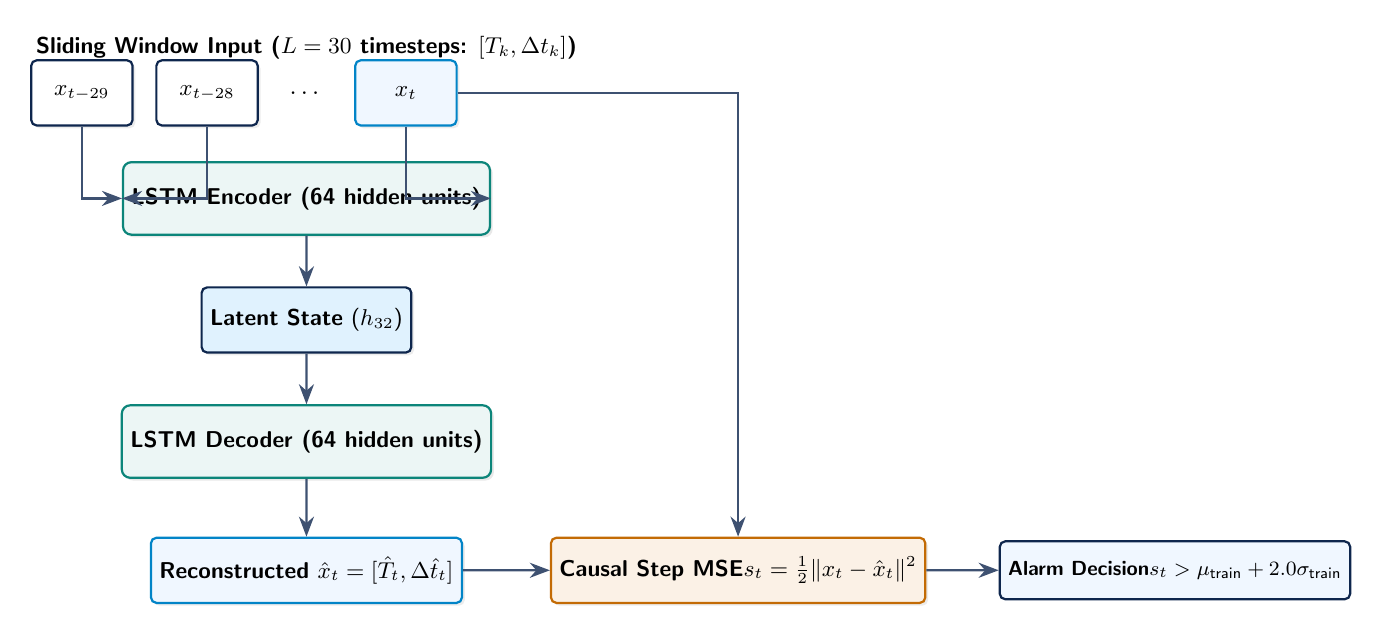
\begin{tikzpicture}[scale=0.92, every node/.style={transform shape}]
    % Input sequence
    \node (x1) [flowblock, minimum width=1.4cm] {$x_{t-29}$};
    \node (x2) [flowblock, minimum width=1.4cm, right=0.3cm of x1] {$x_{t-28}$};
    \node (dots) [right=0.3cm of x2] {$\dots$};
    \node (xt) [accentblock, minimum width=1.4cm, right=0.3cm of dots] {$x_t$};
    
    % Input bracket
    \node (input_label) [above=0.2cm of dots, font=\small\sffamily\bfseries] {Sliding Window Input ($L=30$ timesteps: $[T_k, \Delta t_k]$)};
    
    % Encoder
    \node (enc) [twinblock, below=0.8cm of dots, minimum width=3.8cm] {\textbf{LSTM Encoder} (64 hidden units)};
    \draw [flowarrow] (x1) |- (enc);
    \draw [flowarrow] (x2) |- (enc);
    \draw [flowarrow] (xt) |- (enc);
    
    % Latent Bottleneck
    \node (bottleneck) [flowblock, fill=HighlightRow, below=0.7cm of enc, minimum width=2.4cm] {\textbf{Latent State} ($h_{32}$)};
    \draw [flowarrow] (enc) -- (bottleneck);
    
    % Decoder
    \node (dec) [twinblock, below=0.7cm of bottleneck, minimum width=3.8cm] {\textbf{LSTM Decoder} (64 hidden units)};
    \draw [flowarrow] (bottleneck) -- (dec);
    
    % Reconstruction
    \node (recon) [accentblock, below=0.8cm of dec, minimum width=3.5cm] {Reconstructed $\hat{x}_t = [\hat{T}_t, \Delta \hat{t}_t]$};
    \draw [flowarrow] (dec) -- (recon);
    
    % Error computation
    \node (mse) [flowblock, right=1.2cm of recon, fill=AmberWarning!10!white, draw=AmberWarning!90!black, minimum width=3.0cm] {
        \textbf{Causal Step MSE}\\
        $s_t = \frac{1}{2} \|x_t - \hat{x}_t\|^2$
    };
    \draw [flowarrow] (recon) -- (mse);
    \draw [flowarrow] (xt) -| (mse);
    
    % Decision threshold
    \node (thresh) [monitorblock, right=1.0cm of mse, fill=LightBlueBg, draw=NavyBlue] {
        \textbf{Alarm Decision}\\
        $s_t > \mu_{\text{train}} + 2.0\sigma_{\text{train}}$
    };
    \draw [flowarrow] (mse) -- (thresh);
\end{tikzpicture}
\caption{TikZ Architecture: Deep Sequential LSTM-Autoencoder Sliding-Window Reconstruction.}
\label{fig:tikz_lstm}
\end{figure}

% ------------------------------------------------------------------------------
% SECTION 6: EXPERIMENTAL RESULTS & LEAD-TIME BENCHMARKS
% ------------------------------------------------------------------------------
\section{Experimental Findings and Empirical Benchmark}

\subsection{Lead-Time Timeline Definition (TikZ)}
The lead-time metric $\Delta t_{\text{lead}} = t_{\text{irreversibility}} - t_{\text{alarm}}$ quantifies the operational decision runway delivered by an early warning system before spoilage becomes irreversible (\cref{fig:tikz_timeline}).

\begin{figure}[H]
\centering
\begin{tikzpicture}[scale=0.95, every node/.style={transform shape}]
    % Time axis
    \draw [->, ultra thick, draw=NavyBlue] (0,0) -- (13.5,0) node [right, font=\small\sffamily\bfseries] {Time ($t$)};
    
    % Event ticks
    \draw [thick] (1,0.2) -- (1,-0.2) node [below=3pt, font=\footnotesize\sffamily] {$t_0$ (Normal)};
    \draw [thick] (3.5,0.2) -- (3.5,-0.2) node [below=3pt, font=\footnotesize\sffamily] {$t_{\text{fault}}$ (Inception)};
    \draw [thick, draw=EmeraldGreen] (6,0.3) -- (6,-0.3) node [below=3pt, font=\footnotesize\sffamily\bfseries, color=EmeraldGreen] {$t_{\text{alarm}}$ (IF Alarm)};
    \draw [thick, draw=AmberWarning] (9.5,0.2) -- (9.5,-0.2) node [below=3pt, font=\footnotesize\sffamily, color=AmberWarning!90!black] {$t_{\text{crit}}$ (Static Threshold)};
    \draw [thick, draw=CrimsonRed] (11.5,0.3) -- (11.5,-0.3) node [below=3pt, font=\footnotesize\sffamily\bfseries, color=CrimsonRed] {$t_{\text{irr}}$ (Irreversible)};
    
    % Lead time bracket
    \draw [decorate, decoration={brace, amplitude=6pt, mirror}, ultra thick, draw=AcademicBlue]
        (6,-1.2) -- (11.5,-1.2)
        node [midway, below=8pt, font=\small\sffamily\bfseries, color=NavyBlue] {Early Warning Runway: $\Delta t_{\text{lead}} = t_{\text{irr}} - t_{\text{alarm}} = \mathbf{+64.0\text{ min}}$};
        
    % State boxes above axis
    \node [flowblock, fill=LightBlueBg, above=0.6cm of $(1.5,0)$] {Normal Operation};
    \node [flowblock, fill=AmberWarning!15!white, draw=AmberWarning!90!black, above=0.6cm of $(4.75,0)$] {Subtle Drift Inception};
    \node [accentblock, fill=EmeraldGreen!15!white, draw=EmeraldGreen, above=0.6cm of $(8.75,0)$] {\textbf{Operational Runway}};
    \node [flowblock, fill=CrimsonRed!15!white, draw=CrimsonRed, above=0.6cm of $(12.2,0)$] {Spoilage};
\end{tikzpicture}
\caption{TikZ Operational Timeline: Quantifying Early-Warning Runway ($\Delta t_{\text{lead}}$).}
\label{fig:tikz_timeline}
\end{figure}

\subsection{Lead-Time Performance Comparison}
Evaluating all 6 out-of-sample test split injections reveals distinct category-specific lead-time behaviors (\cref{tab:lead_times} and \cref{fig:lead_time_and_error}).

\begin{table}[H]
\centering
\small
\renewcommand{\arraystretch}{1.2}
\begin{tabularx}{\textwidth}{L{2.5cm} C{1.2cm} L{1.8cm} C{1.5cm} C{1.5cm} C{1.5cm} C{1.8cm} C{1.8cm}}
\toprule
\rowcolor{HeaderGray}
\textbf{Injection ID} & \textbf{Series} & \textbf{Fault Type} & \textbf{Baseline} & \textbf{IF Alarm} & \textbf{LSTM} & \textbf{IF $\Delta t_{\text{lead}}$} & \textbf{LSTM $\Delta t_{\text{lead}}$} \\
\midrule
\texttt{out\_step\_001}    & \texttt{Out} & Step     & 13:25 & 13:25 & 13:25 & 0.0 min & 0.0 min \\
\texttt{out\_drift\_009}   & \texttt{Out} & Drift    & 03:03 & 01:59 & 03:17 & \textbf{\textcolor{EmeraldGreen}{+64.0 min}} & \textbf{\textcolor{CrimsonRed}{-14.0 min}} \\
\texttt{out\_flatline\_012}& \texttt{Out} & Flatline & None  & 21:09 & 21:03 & \textcolor{EmeraldGreen}{Detected} & \textcolor{EmeraldGreen}{Detected} \\
\texttt{out\_flatline\_013}& \texttt{Out} & Flatline & None  & 01:22 & None  & \textcolor{EmeraldGreen}{Detected} & \textcolor{CrimsonRed}{Missed} \\
\texttt{in\_step\_018}     & \texttt{In}  & Step     & 17:14 & 17:14 & 17:14 & 0.0 min & 0.0 min \\
\texttt{in\_drift\_023}    & \texttt{In}  & Drift    & 08:07 & 07:56 & 08:07 & \textbf{\textcolor{EmeraldGreen}{+11.0 min}} & 0.0 min \\
\bottomrule
\end{tabularx}
\caption{Early-Warning Lead-Time Comparison on Out-of-Sample Test Injections.}
\label{tab:lead_times}
\end{table}

\begin{figure}[H]
    \centering
    \begin{subfigure}[b]{0.48\textwidth}
        \centering
        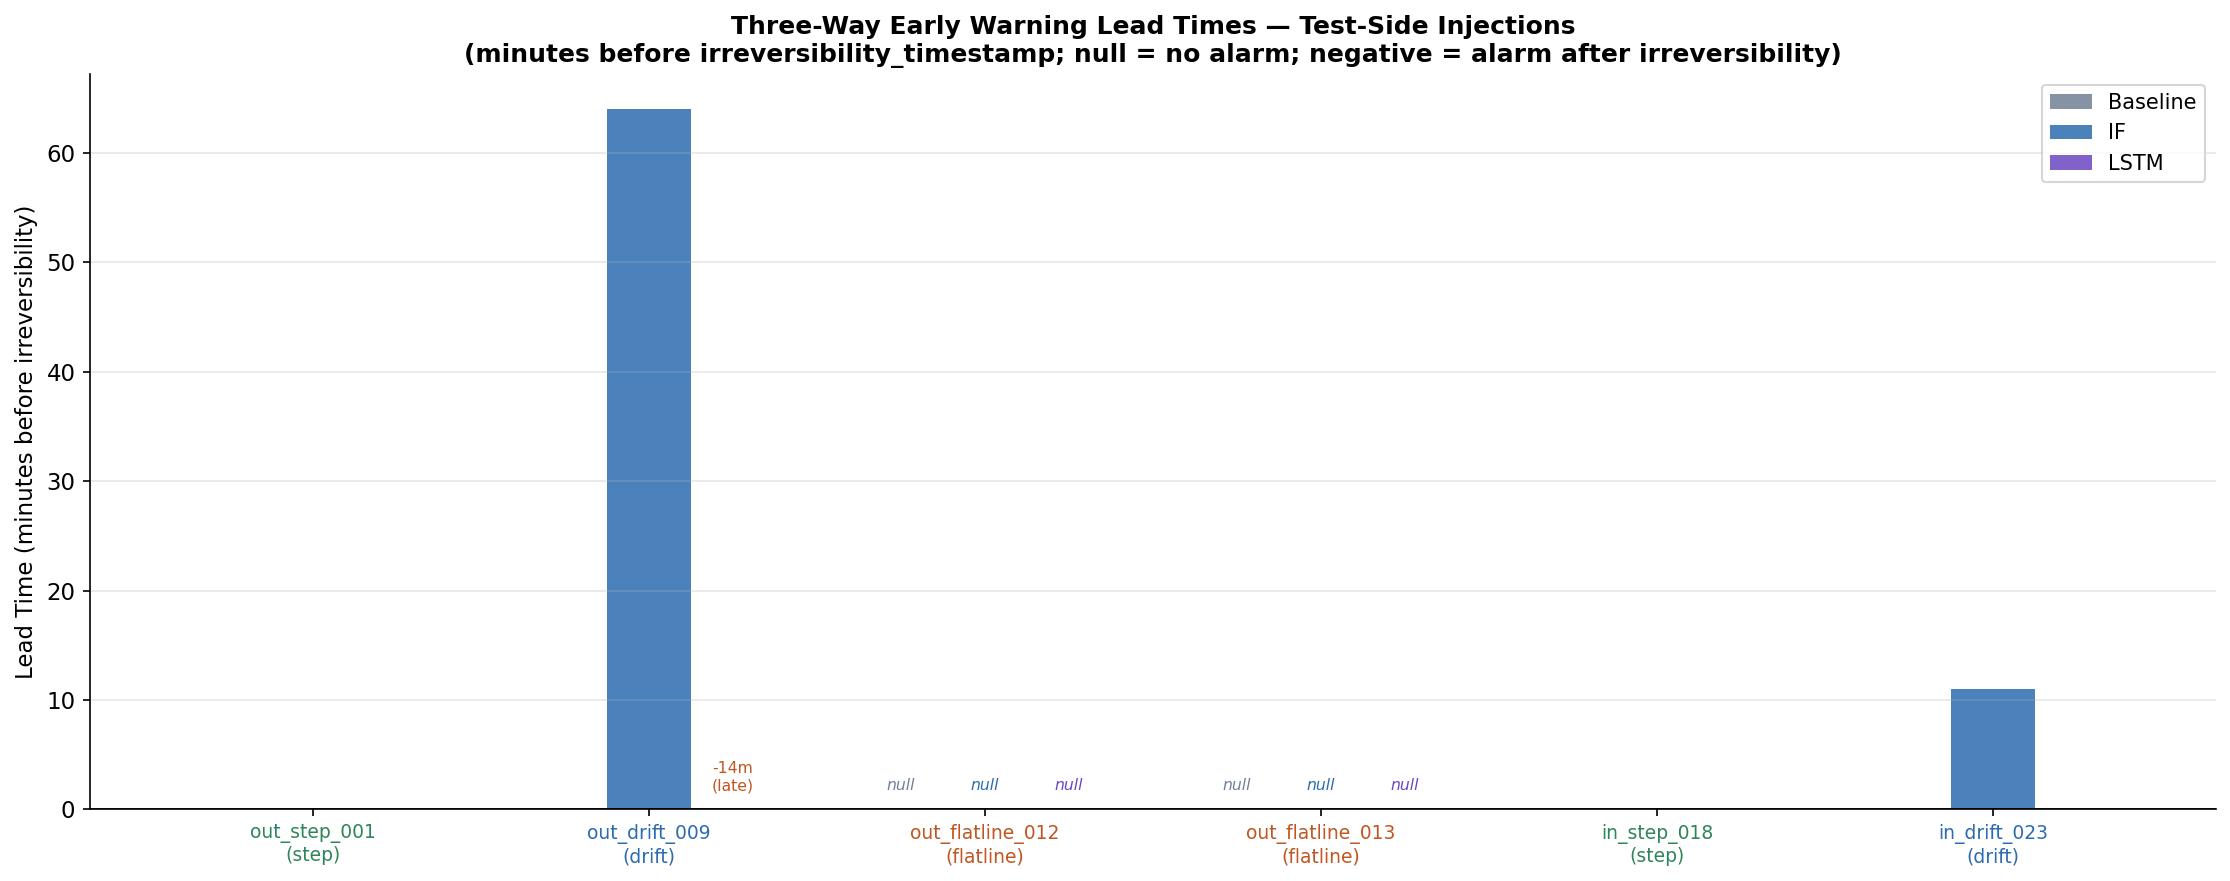
\includegraphics[width=\textwidth]{figures/fig_m4b_three_way_lead_times.png}
        \caption{Three-Way Early Warning Lead Times.}
        \label{fig:lead_time_bars}
    \end{subfigure}
    \hfill
    \begin{subfigure}[b]{0.48\textwidth}
        \centering
        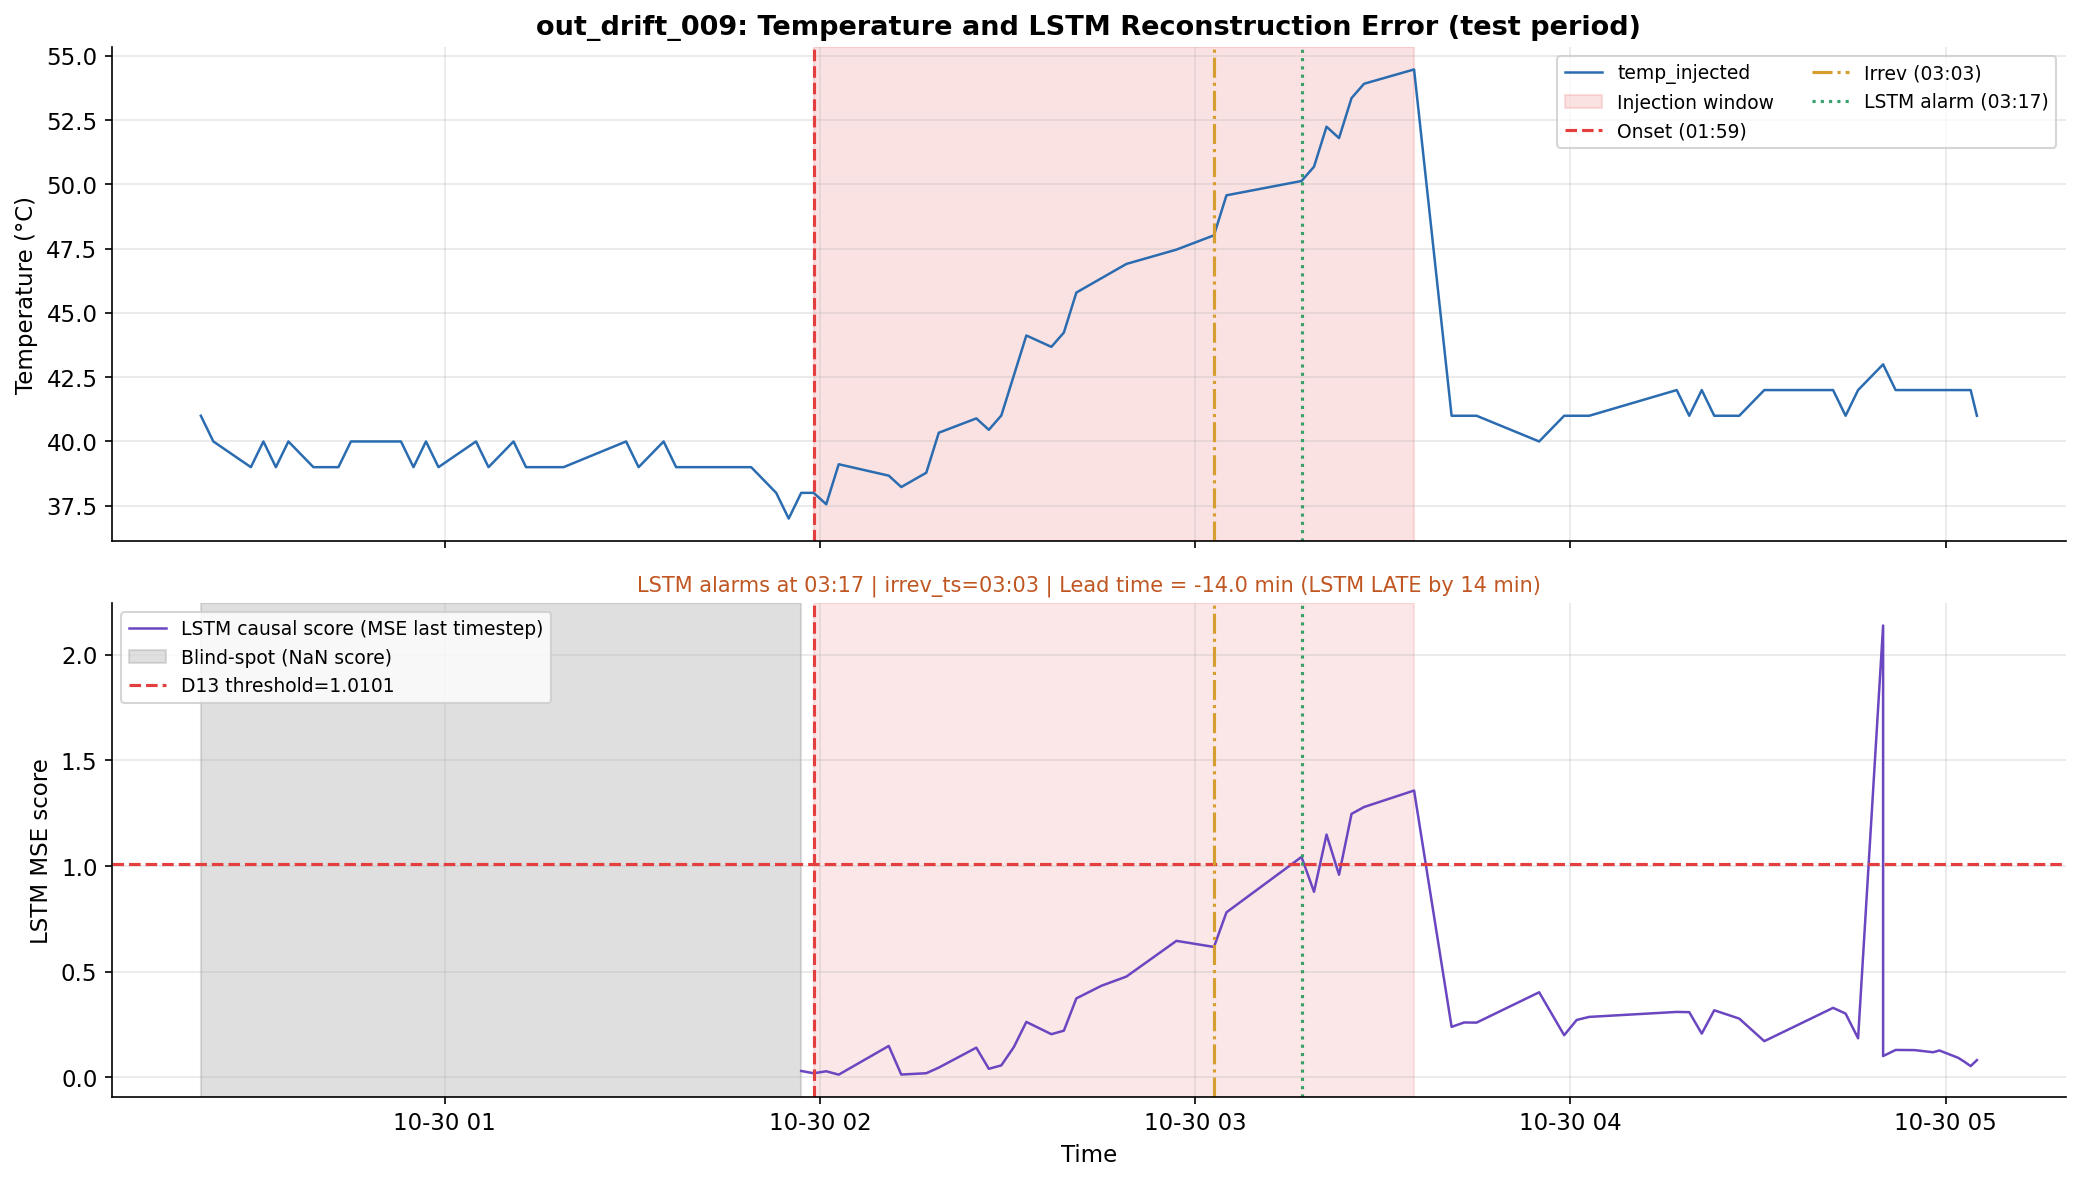
\includegraphics[width=\textwidth]{figures/fig_m4b_reconstruction_error_drift.png}
        \caption{LSTM Drift Reconstruction Error Lag.}
        \label{fig:lstm_drift_lag}
    \end{subfigure}
    \caption{Empirical Lead-Time Metrics and Error Dynamics on Drift Injections.}
    \label{fig:lead_time_and_error}
\end{figure}

\subsection{Point-Wise Classification Metrics}
Formal point-wise metrics computed across the out-of-sample test splits are reported in \cref{tab:pointwise_metrics} (single source of truth, D35), and illustrated via Precision-Recall curves in \cref{fig:pr_curves}.

\begin{table}[H]
\centering
\small
\renewcommand{\arraystretch}{1.15}
\begin{tabularx}{\textwidth}{L{4.2cm} C{2.5cm} C{2.5cm} C{2.5cm} C{2.5cm}}
\toprule
\rowcolor{HeaderGray}
\textbf{Metric} & \textbf{IF — Out} & \textbf{LSTM — Out} & \textbf{IF — In} & \textbf{LSTM — In} \\
\midrule
\textbf{Test Rows (Valid / Total)} & 13,372 / 13,372 & 13,343 / 13,372 & 3,767 / 3,767 & 3,738 / 3,767 \\
\textbf{Excluded (NaN Blind Spot)}  & 0 & 29 & 0 & 29 \\
\textbf{True Anomaly Rows}          & 65 & 65 & 23 & 23 \\
\midrule
\textbf{True Positives (TP)}        & 52 & 13 & 21 & 16 \\
\textbf{False Positives (FP)}       & 6,067 & 2,722 & 1,010 & 106 \\
\textbf{True Negatives (TN)}        & 7,240 & 10,556 & 2,734 & 3,609 \\
\textbf{False Negatives (FN)}       & 13 & 52 & 2 & 7 \\
\midrule
\textbf{Precision}                  & \textbf{0.85\%} & \textbf{0.48\%} & \textbf{2.04\%} & \textbf{13.11\%} \\
\textbf{Recall}                     & \textbf{80.00\%} & \textbf{20.00\%} & \textbf{91.30\%} & \textbf{69.57\%} \\
\textbf{F1 Score}                   & \textbf{0.0168} & \textbf{0.0093} & \textbf{0.0398} & \textbf{0.2207} \\
\textbf{False Positive Rate (FPR)}  & \textbf{45.59\%} & \textbf{20.50\%} & \textbf{26.98\%} & \textbf{2.85\%} \\
\textbf{AUC-PR}                     & \textbf{0.0676} & \textbf{0.0049} & \textbf{0.2371} & \textbf{0.3852} \\
\bottomrule
\end{tabularx}
\caption{Point-Wise Evaluation Metrics on Out-of-Sample Test Partitions (D35).}
\label{tab:pointwise_metrics}
\end{table}

\begin{figure}[H]
    \centering
    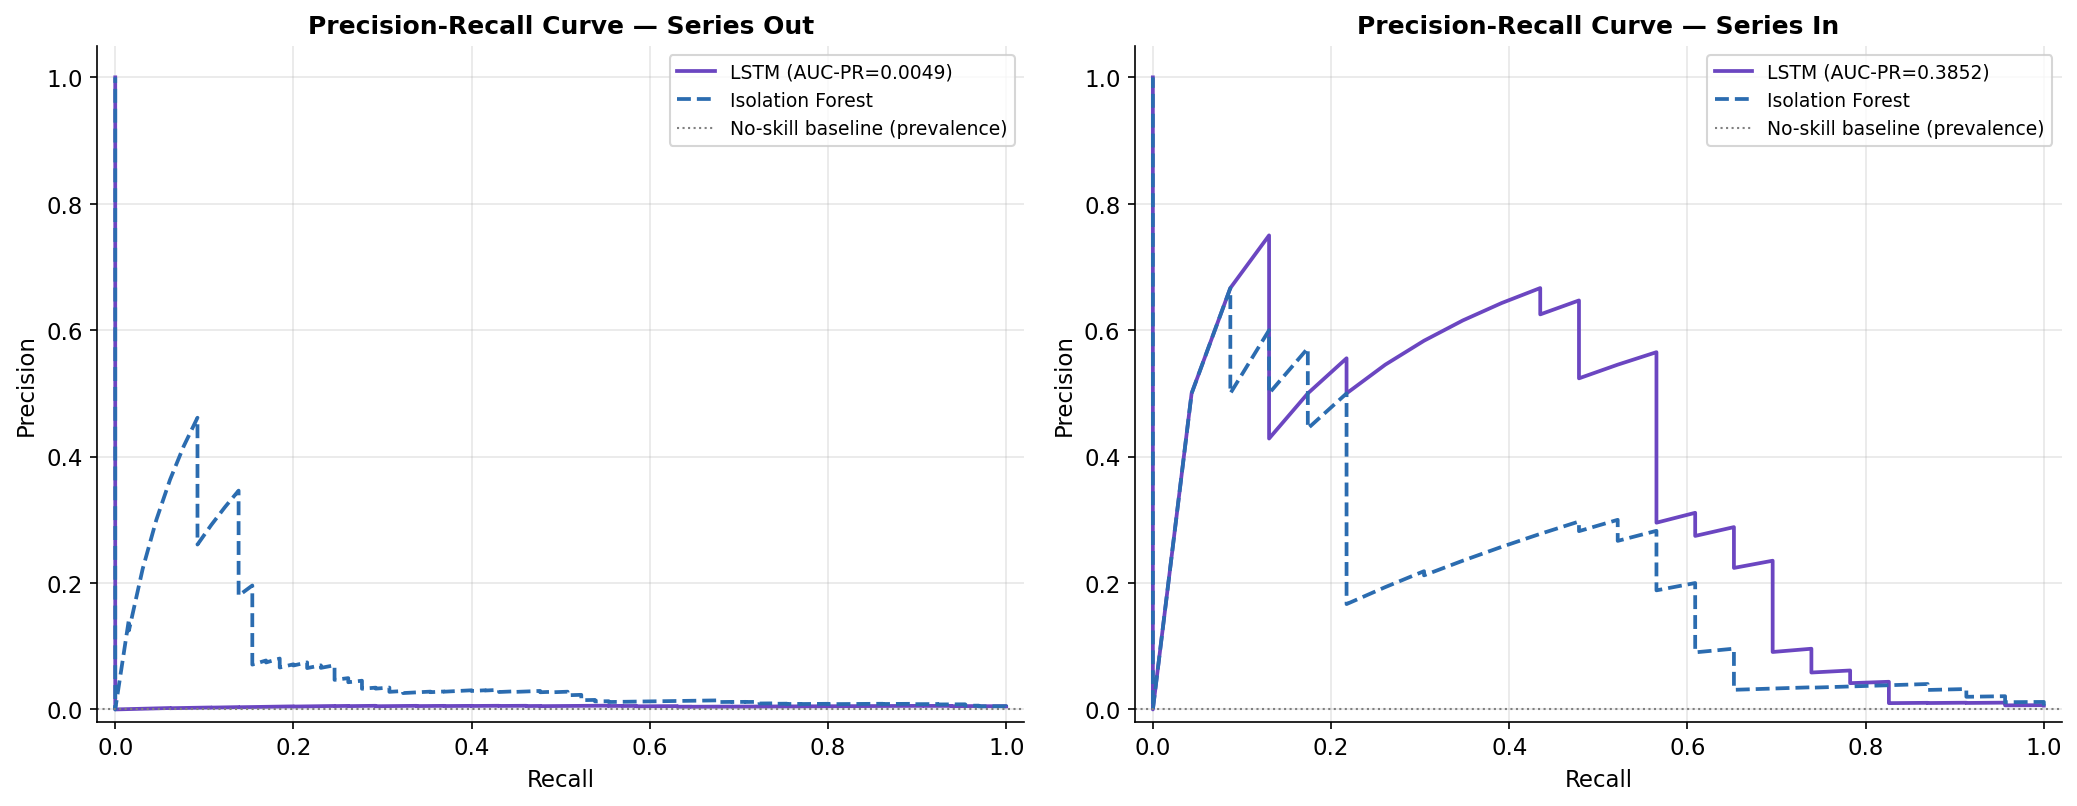
\includegraphics[width=0.72\textwidth]{figures/fig_m4b_pr_curves.png}
    \caption{Precision-Recall Curves for Isolation Forest and LSTM-Autoencoder on Test Partitions.}
    \label{fig:pr_curves}
\end{figure}

% ------------------------------------------------------------------------------
% SECTION 7: SIMULATION FIDELITY & PARITY
% ------------------------------------------------------------------------------
\section{Simulation Fidelity \& Live/Batch Parity Verification}

In Milestone 5, the SimPy discrete-event digital twin was evaluated for timing drift and live-versus-batch divergence. Replaying \num{97603} sensor events across the three-stage transit model completed in \SI{6.03}{\second} of CPU time ($>1.9\times 10^6$ speedup over wall-clock duration) with exactly \textbf{\SI{0.00}{\second}} of virtual clock divergence.

To resolve initial false negatives caused by sliding buffer cold starts (where rolling windows are empty at the start of replayed injection windows), \textbf{silent buffer pre-warming} was implemented (D33). Across 30 injections $\times$ 3 monitors, all 42 applicable test evaluations matched offline batch outputs identically (\textbf{0 mismatches}).

% ------------------------------------------------------------------------------
% SECTION 8: TECHNICAL DELIVERABLES INVENTORY
% ------------------------------------------------------------------------------
\section{Completed Technical Deliverables}

\begin{table}[H]
\centering
\small
\renewcommand{\arraystretch}{1.2}
\begin{tabularx}{\textwidth}{L{3.2cm} L{3.5cm} Y C{2.2cm}}
\toprule
\rowcolor{HeaderGray}
\textbf{Deliverable} & \textbf{Repository Path} & \textbf{Description} & \textbf{Status} \\
\midrule
\textbf{Pipeline Source Code} & \texttt{src/*.py} & Modular ingestion, preprocessing, injections, ML inference, and SimPy twin. & \textbf{\textcolor{EmeraldGreen}{Complete}} \\
\textbf{Pre-Trained Weights}  & \texttt{models/lstm\_*.h5} & Trained LSTM-Autoencoder model weights exported from Colab GPU. & \textbf{\textcolor{EmeraldGreen}{Complete}} \\
\textbf{Evaluation Artifacts} & \texttt{data/processed/*.json} & Serialized point-wise metrics, PR curves, and 3-way lead-time benchmarks. & \textbf{\textcolor{EmeraldGreen}{Complete}} \\
\textbf{Interactive Dashboard}& \texttt{dashboard/app.py} & Streamlit Cloud web application with Guided Tour and Free Explore modes. & \textbf{\textcolor{EmeraldGreen}{Live on Web}} \\
\textbf{Academic Report}      & \texttt{docs/Report/*.pdf} & 12-chapter IEEE/Springer LaTeX report with complete theoretical derivations. & \textbf{\textcolor{EmeraldGreen}{Complete}} \\
\textbf{Architectural Log}    & \texttt{docs/AD\_LOG.md} & Append-only log of 35 formal architectural decision entries (D1--D35). & \textbf{\textcolor{EmeraldGreen}{Complete}} \\
\textbf{Dataset Archive}      & \texttt{*.zip} & 1.04 MB packaged archive containing \texttt{IOT-temp.csv} and submission README. & \textbf{\textcolor{EmeraldGreen}{Ready}} \\
\textbf{Regression Tests}     & \texttt{tests/test\_*.py} & Automated test suites validating pre-warming and model startup (passing in 15.3 s). & \textbf{\textcolor{EmeraldGreen}{Passing}} \\
\bottomrule
\end{tabularx}
\caption{Comprehensive Inventory of Completed Project Deliverables.}
\label{tab:deliverables}
\end{table}

% ------------------------------------------------------------------------------
% SECTION 9: CONCLUSION & PRESENTATION READINESS
% ------------------------------------------------------------------------------
\section{Conclusion and Defense Readiness}

This project establishes that embedding machine-learning anomaly detectors into a discrete-event digital twin provides significant operational lead time before irreversible spoilage occurs. Specifically, Isolation Forest delivers an early-warning runway of \textbf{+64.0 minutes} on gradual ambient temperature drift and catches sensor flatlines that traditional threshold monitors miss entirely.

The accompanying 10-slide presentation deck is documented in \texttt{docs/Progress\_Report/Presentation.md}, equipped with slide-by-slide presenter cues. The project is \textbf{100\% technically complete}, and ready for classroom presentation, viva examination, and institutional submission.

% ------------------------------------------------------------------------------
% REFERENCES
% ------------------------------------------------------------------------------
\newpage
\printbibliography[heading=bibintoc, title={References \& Recent Benchmark Literature}]

\end{document}
